\section{Design}
\label{sec:design}

Our \xxx prototype is designed to debug performance issues in complex modern applications.
It performs lightweight full system tracing of every process including system calls, interprocess messages, and MacOS system daemons.
Offline, we build a graph based on thread executions, with nodes defined by per-request execution segments, and edges wherever there are temporal constraints between threads of execution.

\begin{figure*}[tb]
    \centering
    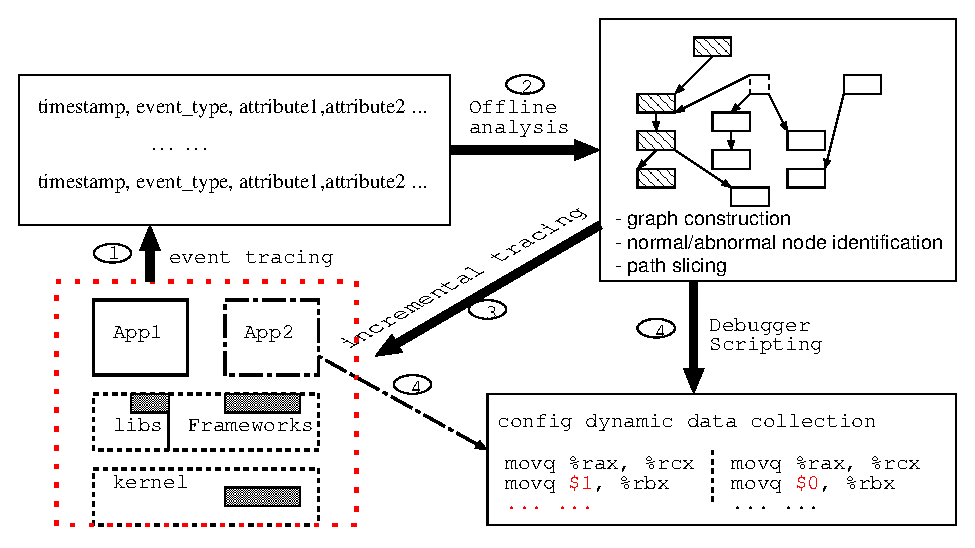
\includegraphics[width=0.7\linewidth]{ArgusOverview.eps}
    \caption{Design Overview}
    \label{fig:argus-overview}
\end{figure*}

\subsection{Use Cases}

\xxx can be used in two primary ways:
\begin{enumerate}
    \item \xxx can continuously run live in the background and collect full
    system logs. The user works as usual until a crash or performance issue is
    observed.

    \item The user can begin with a reproducible performance issue, no matter how often it appears, and collect
    logs in two situations: a) a baseline situation where the program runs
    normally, and b) a spinning situation that exposes the performance issue.

\end{enumerate}
For a simple issue, like a rare segmentation fault, just having \xxx's lightweight logs may be enough to perform a diagnosis.
However, in most cases, \xxx will need to be used interactively, so the user needs to be able to
%restart the affected application and
reproduce the problem on demand.
The user can request more detailed logs in several ways, then reproduce the problem, and gather enough data to narrow in even further on the issue.
The general process for interactive debugging with \xxx is as follows:
\begin{enumerate}
    \item First, the user finds the node \emph{$N_{spin}$} in the \xxx graph
    that corresponds to a hanging thread of execution. The user may leverage
    the system clock time to search for events (\eg, keystrokes).

    \item Next, the user attempts to find the node in the normal case that
    corresponds with $N_{spin}$. There will likely be many possible candidates
    at first, so the user can narrow in on specific nodes and gather more
    detailed information in that area of the program.

    \item Now, with knowledge of $N_{spin}$ and (a small number of) matching
    nodes in the normal graph, the user performs a backward slice through the
    graphs to attempt to find the defining difference between the cases. This
    difference should accurately predict whether a given log represents a
    normal or spinning case, and usually indicates quite directly the root
    cause. As before, additional information may need to be collected from
    certain points in the program to be able to distinguish between the cases.

\end{enumerate}
As shown in Figure \ref{fig:argus-overview}, the user's main operations leveraging\xxx toolkits are
a) inspection of the graph,
b) performing slicing on the graph to show dependent nodes,
c) comparing graph slices between normal and spinning cases, and
d) selecting a graph node to gather more information with our debugger scripts.

\subsection{Event Tracing}
The instrumentation in \xxx leverages tracing technology from Apple's event logging infrastructure.
It produces a stream of timestamped events with the following format:

\textit{timestamp, Mach\_msg\_send, local\_port, remote\_port, ...}

An event consists of a timestamp, an event type name to annotate current activity, and arbitrary attributes.

We augment the existing event types with more attributes to support our extensive usage.
For example, the \textit{local\_port and remote\_port} above are added to support our analysis on \textit{ mach\_msg} flow.
Beside, we also add new types of events in kernel and libraries. 
They are logged to a file for offline analysis.

\subsection{Offline Graph Construction}
Compared to Magpie which requires user input event schema, our system defined the event schema to convert the log into relationship graphs.
The event schema defines how a subset of events connect each other, and what events indicates the begin and end of a request.

We generate the graph by taking two steps.
The first step is to link the events with the schema, for example, the event indicats sending message, and the event representing receiving the message, are connected to each other,
The second step is to split the events from the same thread into multiple execution segments, decomplexing the execution of different requests.

However, the graphs constructed with event schema is hard to be accurate and complete, even though our schema has covered all dependency idioms used by tranditional causal tracing.
For instance, the mutex contention, reflected as the thread wailt and wakeup in our system, can be a producer and consumer pattern or an exclusive operation on shared resource. 

\subsection{Incremental Tracing}
The graph generated are subject to users' inspection and improvement.
The inspection tool built upon the graph reports the potential missing and superfluous edges.
Users can optionally check the report and improve the graph by collecting more data.

\xxx provides the ad-hoc command line tool to insert the hareware breakpoints, and a detouring style instrumentation library.
We construct the API to get lightweight call stacks by unwinding the \emph{rbp} in the library.
User can repeating this process and apply the offline tool again to generate the improved graph. 

\subsection{Debugger Scripting}
\xxx can concisely degugging the performance issue with the intraction with users.
we desgin tools upon the graph to perform path slicing and diffing first to narrow down the problem to a fine range.
Users can further enable the concrete debugging with our scripts, which take the output of the last step and conduct steps debugging and callstack sampling within the range to bound overheads.
Diffing is applied again on the debugging logs from boh the normal case and the problematic case.
Mostly the call stacks from the precise range and the branch istructions can reveal the root cause of performance issue.
